%This is a proposed template for a master thesis report for the FH Wiener Neustadt. The present document is free.

%You can redistribute it and/or modify it under the terms of the GNU General Public License as published by the Free Software Foundation; either version 2 of the License, or (at your option) any later version.

% Author: Joan Miralles
% Datum: 05/04/2015
% Latest update: 11/07/2016
%version: 2.2

%   Study Thesis:   Write here your title
%   Institution:    Fachhochschule Wiener Neustadt
%   Topic:          Whatever you want to write about
%   Author:         Name Name Name
%   Date:           01/04/2015
%   Version:        1.0    

        %----------------------------------------------------%
\documentclass[oneside,12pt,bibliography=totoc]{scrbook}

\subject{Master's Thesis}
\title{An analysis of share movement and sentiment of tweets: detailed analysis of automotive companies.}
%\subtitle{A fiction story telling the truth}
\author{David Kovacs, MSc}
%\publishers{Published by the publisher\\ at a secret location}
%\extratitle{Stories of ducks}
%\uppertitleback{\vspace{3cm}I want to thank Scrooge MacDuck for his financial Support}
\date{\today}

%'oneside' specifies that the pages will be printed on one sides of a every page. If you want to print on both sides of your pages use the parameter 'twoside'. Remember to order the printing job on one side of every page!!!


    %%%%------------------PREAMBLE----------------%%%%
    %%----------------------------------------------%%

    %%%%%-------------------PACKAGES-----------------%%%%% 
    
%\usepackage[utf8]{inputenc}
\usepackage[a4paper,top=25mm,bottom=30mm,left=30mm,right=25mm]{geometry}   %allows to change margins and distances within the page's frame. Be careful with this tool. Remember to delete the frame!!!!

%\usepackage{showframe}
%\usepackage[english]{babel}    %the package babel is not necessary as long as you write your thesis in English.
%\usepackage{csquotes}
\usepackage{graphicx}   %loads the graphics package, necessary for pictures
\usepackage{url}
%\usepackage{wallpaper}
\usepackage{hyperref}   %Automatically turn all your internal references into hyperlinks.
\makeatletter
\hypersetup{pdfinfo={
  Title=\@title,
  Author=\@author,
  Subject=Master's Thesis,
  Keywords={EMH,Twitter,Sentiment}}
}
\makeatother

\usepackage[toc,page]{appendix}
\usepackage[final]{pdfpages}
\usepackage{soul}       %provides hyphenatable letterspacing, underlining and some derivatives such as everstriking and highlighting.
%\usepackage[intoc]{nomencl}   %helps to format a nomenclature.
%\makenomenclature

\usepackage[printonlyused, withpage]{acronym}

\usepackage[UKenglish]{isodate} %Provides the format for the date on the title page. Read the package documentation for all the possible date formats.

\usepackage{array}
\usepackage{longtable}

%\usepackage{lipsum}
\usepackage{caption}
%\usepackage{abstract}   %This package allows to modify the Abstract style, position and font. Defines the abstract automatically.
\usepackage{supertabular}
\usepackage{tabto}

\usepackage{fontspec}
\setmainfont{MyFont.TTF}%
[Ligatures=TeX,
    Path=fonts/,
    BoldFont=MyFont_Bold.TTF,
    ItalicFont=MyFont_Italic.TTF,
    BoldItalicFont=MyFont_BoldItalic.TTF]


\usepackage{xcolor}
\definecolor{header-blue}{RGB}{22,48,114}

\setcounter{secnumdepth}{4}

\usepackage{titlesec}

\titleformat{\chapter}[hang]{\bfseries\Large\color{header-blue}}{\makebox[.63cm][l]{\thechapter.}}{0pt}{}[]
\titlespacing*{\chapter}{0pt}{18pt}{12pt}

\titleformat{\section}[hang]{\bfseries\large\color{header-blue}}{\makebox[1.27cm][l]{\thesection}}{0pt}{}[]
\titlespacing*{\section}{0pt}{6pt}{12pt}

\titleformat{\subsection}[hang]{\bfseries\normalsize\color{header-blue}}{\makebox[1.5cm][l]{\thesubsection}}{0pt}{}[] 
\titlespacing*{\subsection}{0pt}{6pt}{12pt}

\titleformat{\subsubsection}[hang]{\bfseries\normalsize\color{header-blue}}{\makebox[1.5cm][l]{\thesubsubsection}}{0pt}{}[]
\titlespacing*{\subsubsection}{0pt}{6pt}{12pt}

\titleformat{\paragraph}[hang]{\bfseries\normalsize\color{header-blue}}{\makebox[2.5cm][l]{\theparagraph}}{0pt}{}[]
\titlespacing*{\paragraph}{0pt}{6pt}{12pt}

%\usepackage{footnote}      %Just in case you want to include footnotes
%\usepackage{indentfirst}    %Indent in every first paragraph after \chapter and \section.
\usepackage[onehalfspacing]{setspace}      %Change spacing easily with simple commands

\usepackage{amsmath}       %This package introduces several new commands that are more powerful and flexible than the ones provided by LaTeX. Uncomment them if you are using complex mathematical notation.
\usepackage{mathtools}     %The mathtools package fixes some amsmath quirks and adds some useful settings, symbols, and environments to amsmath.

\usepackage{cleveref}

\graphicspath{{images/}}    %Direction where LaTeX will look for the images.
\DeclareGraphicsExtensions{.pdf,.png,.jpg,.mps}

\usepackage[backend=bibtex,style=numeric,citestyle=numeric-comp]{biblatex}
\addbibresource{references.bib}     %Imports bibliography file

\clubpenalty = 10000 
\widowpenalty = 10000
\displaywidowpenalty = 10000

\definecolor{mygreen}{rgb}{0,0.6,0}
\definecolor{mygray}{rgb}{0.5,0.5,0.5}
\definecolor{mylightgray}{rgb}{0.9,0.9,0.9}
\definecolor{mymauve}{rgb}{0.58,0,0.82}

\usepackage{listings}

\lstset{ %
  %backgroundcolor=\color{mylightgray},   % choose the background color; you must add \usepackage{color} or \usepackage{xcolor}
  basicstyle=\footnotesize,        % the size of the fonts that are used for the code
	%basicstyle=\small\sffamily,
  breakatwhitespace=false,         % sets if automatic breaks should only happen at whitespace
  breaklines=true,                 % sets automatic line breaking
  captionpos=t,                    % sets the caption-position to bottom
  commentstyle=\color{mygreen},    % comment style
  deletekeywords={...},            % if you want to delete keywords from the given language
  escapeinside={\%*}{*)},          % if you want to add LaTeX within your code
  extendedchars=true,              % lets you use non-ASCII characters; for 8-bits encodings only, does not work with UTF-8
  frame=tb,                    % adds a frame around the code
  keepspaces=true,                 % keeps spaces in text, useful for keeping indentation of code (possibly needs columns=flexible)
  keywordstyle=\color{blue},       % keyword style
  %language=Octave,                 % the language of the code
  morekeywords={*,...},            % if you want to add more keywords to the set
  numbers=left,                    % where to put the line-numbers; possible values are (none, left, right)
  numbersep=5pt,                   % how far the line-numbers are from the code
  numberstyle=\tiny\color{mygray}, % the style that is used for the line-numbers
  rulecolor=\color{black},         % if not set, the frame-color may be changed on line-breaks within not-black text (e.g. comments (green here))
  showspaces=false,                % show spaces everywhere adding particular underscores; it overrides 'showstringspaces'
  showstringspaces=false,          % underline spaces within strings only
  showtabs=false,                  % show tabs within strings adding particular underscores
  stepnumber=2,                    % the step between two line-numbers. If it's 1, each line will be numbered
  stringstyle=\color{mymauve},     % string literal style
  tabsize=2,                       % sets default tabsize to 2 spaces
  title=\lstname                   % show the filename of files included with \lstinputlisting; also try caption instead of title
}

\renewcommand{\labelitemii}{-}
\renewcommand{\labelitemi}{--}

    %%%------------- Page Layout Settings ----------------------%
%%---Just in case you want to customize the page layout-----
%\setlength{\topmargin}{0mm} 
%\setlength{\textheight}{225mm} 
%\setlength{\oddsidemargin}{4,6mm} 
%\setlength{\evensidemargin}{4,6mm}
%\setlength{\textwidth}{150mm} 
%\setlength{\headheight}{15pt}

    %%%%----------------Paragraphs formatting---------------------%%%%%
%\linespread{1.0}    %Line spacing, only accepts values 1.0, 1.3 and 1.6. If set here, it will apply to the whole document, including ToC, Lists...
%\setlength{\baselineskip}{5mm} %%minimum space between the bottom of two successive lines in a paragraph
%\setlength{\parindent}{1.25cm}  %Determining paragraph indentation
%\setlength{\parskip}{2mm}   %Determining space between paragraph and preceeding text. This can be set in the preamble or later in the document part, but be careful. If set here, it will apply to the whole document, including ToC, Lists...

    %------------------------- Caption Setup -----------------------%
%\captionsetup{margin=10pt, font=small, labelfont=bf, labelsep=period}

    %-------------------Footnote Setup---------------------%
%\makesavenoteenv{tabular}

    %%%------------------END OF THE PREAMBLE-----------------%%%
    %%--------------------------------------------------------%%

    %------------------------DOCUMENT-----------------------------%

\begin{document}

    %----------------------------FRONT MATTER---------------------%
\frontmatter

% !TeX root = ../main.tex

\makeatletter

\begin{titlepage}

  
\includegraphics[width=6cm]{images/fhwn-logo.png}

  \vspace{70pt}
  {\noindent \linespread{1.3} \color{header-blue} \Huge \textbf{\@title} \par }
  \vspace{5pt}
  {\noindent\LARGE Master's Thesis \par}
  \vspace{20pt}

  \hspace{-35mm}
  
\includegraphics[width=18.67cm]{images/titlepage-line.png}

  \vspace{15pt}

  \tabto{2cm}Submitted by: \tabto{7cm}\textbf{\@author} \\
  \tabto{2cm}Matriculation No.: \tabto{7cm}\textbf{00851488} \\
  \vspace{15pt}
  \tabto{2cm}at \tabto{7cm}\textbf{Master's Programme}\\
  \tabto{7cm}\textbf{Informatics}
  \tabto{7cm}\textbf{Software Architecture and Design} \\
  \vspace{15pt}
  \tabto{2cm}Advisor: \tabto{7cm}\textbf{Priv.-Doz. Dr. Dr. Ingo Feinerer}

  \vfill

  Wiener Neustadt, \today
      
\end{titlepage}
\makeatother

%\renewcommand{\arraystretch}{1}

\vspace{150pt}

\begin{center}
{\noindent\fontsize{18pt}{21.6pt}\color{header-blue}\textbf{DECLARATION OF INTEGRITY}}
\end{center}

\vspace{30pt}

\noindent
I hereby affirm that this research work was written solely by me and that I have not previously submitted this work at another educational institution for the purpose of receiving an academic degree. In particular, contributions by other persons in this work have been appropriately cited and the data gathered through the methods described have been accurately reproduced.
\\

\noindent
Ich erkläre an Eides statt, dass diese Arbeit ausschließlich von mir selbst verfasst wurde und ich diese Arbeit nicht zuvor an einer anderen Bildungseinrichtung zum Zwecke der Erlangung eines akademischen Grades vorgelegt habe. Insbesondere wurden Beiträge anderer Personen entsprechend kenntlich gemacht sowie die in dieser Arbeit verwendeten Daten entsprechend der dargestellten Verfahren gewonnen und richtig wiedergegeben.

\vspace{130pt}

\begin{center}
\begin{tabular}{p{4cm} >{\centering}p{3cm} p{1cm} >{\centering}p{6cm}}
    Wiener Neustadt, & \today & &  \\ \cline{2-2} \cline{4-4}
       & Date &  & Signature \\
\end{tabular}
\end{center}

\clearpage


\newcommand*{\AbstractHead}[1]{%
{\noindent\color{header-blue}\Large\textbf{#1}}
\vspace{10pt}\\
}% These command is used to create the Date and Signature fields.

\newcommand*{\SomeSpace}{%
\vspace{\baselineskip}
}

\AbstractHead{Abstract in English}
\noindent
\normalsize
Despite the theory of efficient market hypothesis some researchers suggest that stock prices can at least partly predicted.
Nowadays Twitter contains a public opinion for every topic as it gets more popular.

This Thesis extracts tweets using DMI-TCAT for five automotive manufacturing companies.
In total \num{11565283} tweets have been captured in the time frame between \printdate{2018-02-28} and \printdate{2018-09-07}.
Afterwords several sentiment detection algorithms (\tb{}, \nb{}, \me{} and \svm{}) have been applied to extract indicators for the public opinion.
The indicators are compared with the share price of the companies using Granger analysis.

It is shown that the share prices of \ford{} and \hyundai{} cannot be predicted very well as only one test of the Granger analysis was significant.
Furthermore, both \svm{} and \nb{} classifiers outperformed the \tb{} classifier which was the reference value during the analysis.

% Many studies have been published which are trying to predict the stock market movement.
% The efficient market hypothesis states that the movements depend on news which are per definition not predictable the stock will follow a random walk pattern.
% Nevertheless some researchers suggest that stock prices are at least partly predictable. 
% On the other hand there are many internet users microblogging today on services like Twitter.
% As the count of characters is limited on Twitter users have to be concise about the topic to write.

\SomeSpace
\AbstractHead{Keywords (at least 3, max. 6)}
\normalsize
\noindent
Efficient Market Hypothesis, Stock Price, Twitter, Sentiment Classification

\glsresetall
\SomeSpace

\AbstractHead{Abstract in German}
\noindent
\normalsize
Trotz der Therorie der Effizienten Markt Hypothese meinen manche Forscher, dass Aktienkurse zumindest teilweise vorhergesagt werden können.
Heutzutage ist auf Plattformen wie Twitter zu jedem beliebigen Thema eine Meinung zu finden.

Diese vorliegende Arbeit extrahiert Tweets mittels DMI-TCAT für fünf Automobilhersteller.
Insgesamt wurden 11565283 Tweets in einem Zeitrahmen zwischen 28.02.2018 und 07.09.2018 erfasst.
Im Anschluss wurden vier verschiedene Sentiment Klassifizierungs Alogrithmen (\tb{}, \nb{}, \me{} and \svm{}) auf die gesammelten Tweets angewandt um Indikatoren für die öffentliche Stimmung zu den jeweiligen Firmen zu extrahieren.
Diese Indikatoren wurden mit den Aktienkursen des jeweiligen Unternehmens mittels Granger Analyse verglichen.

Dabei hat sich gezeigt, dass die Aktienkurse von \ford{} und \hyundai{} sehr schlecht vorhergesagt werden konnte, da nur ein einziger Granger Test signifikant war.
Weiters wurde gezeigt, dass die \svm{} und \nb{} Klassifizierungsalgorithmen dem Referenzalgorithmus \tb{} überlegen sind.

\SomeSpace
\AbstractHead{Keywords (at least 3, max. 6)}
\normalsize
\noindent
Effiziente Markt Hypothese, Aktienkurs, Twitter, Sentiment Klassifizierung

\glsresetall

\normalsize

%%--------------It's your choice to include a dedication and/or acknowledgement---------------%%

%\chapter*{Dedication}
%To mum and dad...

%\chapter*{Acknowledgement}
%\input{frontmatter/acknowledgement}

        %%------------------------TABLE OF CONTENTS AND LISTS-------------------%%
        %%----------------------------------------------------------------------%%
        
\tableofcontents    %\thispagestyle{fancy}

%\printnomenclature
\chapter*{List of Acronyms}
\addcontentsline{toc}{chapter}{List of Acronyms}
%%\chapter{Symbolverzeichnis}
%--------------------------------------------------------------------------------------------------%
\subsection*{Symbols}
\normalsize

%\listofnomenclature{lll}  % Include a list of Symbols (a three column table)
\begin{supertabular}{p{6mm}p{45mm}p{25mm}l}\\

% symbol & name & unit \\
$a$ & distance & m \\
$P$ & power & W (Js$^{-1}$) \\
& & \\ % Gap to separate the Roman symbols from the Greek
$\omega$ & angular frequency & rads$^{-1}$ \\

\end{supertabular}

\clearpage
%--------------------------------------------------------------------------------------------------%

\subsection*{Abbreviations}
%--------------------------------------------------------------------------------------------------%
\normalsize
%\thispagestyle{fancy}
\begin{supertabular}{p{20mm}p{2mm}p{5mm}p{3mm}l}\\

AC				&	&			&	&Alternate current\\
DC				&	&			&	&Direct current\\
DLR				&	&			&	&Deutsches Zentrums f\"ur Luft- und Raumfahrt\\
EP				&	&			&	&Electric propulsion\\
EVA				&	&			&	&Extra Vehicular Activity\\
HOKA			&	&			&	&Hofer-Karrer current monitor\\
ILEA				&	&			&	&Institute for Power Electronics and Electrical Drives\\
IPG				&	&			&	&Inductively heated Plasma Generator\\
IPM				&	&			&	&Institute for Problems of Mechanics, Moscow\\
IRS				&	&			&	&Institute of Space Systems, Stuttgart\\
ISS				&	&			&	&International Space Station\\
LAEPT			&	&			&	&Laboratoire Arc Electrique et Plasma Thermiques\\
LEO				&	&			&	&Low Earth Orbit\\
MPD				&	&			&	&Magneto-Plasma Dynamics\\
NASA			&	&			&	&National Astronautics and Space Administration\\
PEEK			&	&			&	&Polyether ether ketone\\
PPT				&	&			&	&Pulsed Plasma Thruster\\
PVC				&	&			&	&Polyvinyl chloride\\
PWT				&	&			&	&Plasma Wind Tunnel\\
RF				&	&			&	&Radio Frequency\\
SWICS			&	&			&	&Solar Wind Ion Composition Spectrometer\\
TPS				&	&			&	&Thermal Protection System\\
VKI				&	&			&	&Von Karman Institute\\

\end{supertabular}
%!TEX root = ../main.tex

\newacronym{EMH}{EMH}{Efficient Market Hypothesis}
\newacronym{ME}{ME}{Maximum Entropy}
\newacronym{NB}{NB}{Naive Bayes}
\newacronym{NLP}{NLP}{Natural Language Processing}
\newacronym{SVM}{SVM}{Support Vector Machines}
\newacronym{TP}{TP}{True Positive}
\newacronym{TN}{TN}{True Negative}
\newacronym{FP}{FP}{False Positive}
\newacronym{FN}{FN}{False Negative}
\newacronym{bow}{bow}{bag of words}

\listoffigures  %\thispagestyle{fancy}
\addcontentsline{toc}{chapter}{List of Figures}

\listoftables   %\thispagestyle{fancy}
\addcontentsline{toc}{chapter}{List of Tables}

\mainmatter

        %--------------------BODY OF THE THESIS--------------------------%
        %%--------------------------------------------------------------%%
%\cleardoublepage
\chapter{Introduction}    
    %!TEX root = ../main.tex

% \section{Section Title}
% \subsection{Subsection}
% \subsubsection{Subsubsection}
% \paragraph{Paragraph}
% \subparagraph{Subparagraph}

% \ul = underline
% \st = strikethrough
% \hl = highlight
% \textbf = bold face
% \textit = italic face
% \textsl = slanted
% \textsf = sans serif

%%%%%%%%%%%%%%%%%%%%%%%%%%%%%%%%%%%%%%%%%%%%%%%%%%%%%%%%%%%%%%%%%%%%%%%%%

This chapter provides an introduction to this thesis.
In \cref{s:introduction-motivation} the general motivation is discussed.
The section is followed by outlining the research goals in \cref{s:introduction-researchgoals}.
\Cref{s:introduction-researchmethodology} gives an insight into research methods used in order to answer the raised research questions.
Finally, \cref{s:introduction-structureofthisthesis} gives an outlook of the structure of the remaining thesis.

\section{Motivation}
\label{s:introduction-motivation}

Many studies have been published which are trying to predict the stock market movement.
As the \ac{EMH} states that financial market movements depend on news, current events and product releases and all these factors will have significant impact on a company's stock value
\cite{fama1965behavior}.
Due the fact that news and current events are unpredictable stock market prices are following a random walk pattern and cannot predicted with more than 50\% accuracy
\cite{Pagolu2016a}.

Many internet users are microblogging nowadays.
Millions of messages are published daily in popular websites which provides microblogging services, such as Twitter, Tumblr and Facebook.
These published messages describing the personal life, opinions or current issues.
The more users are post about products and services they use the more microblogging websites become a valuable source of peoples opinions and sentiments.
Therefore, this data can be used for marketing, social studies and as a measure of public opinion
\cite{Patodkar2016a, Pagolu2016a}.

As most Twitter messages have a maximum length of 140 characters and speaks public opinion on a topic precisely
\cite{Pagolu2016a}.






\section{Research Goals}
\label{s:introduction-researchgoals}



The goal of this research to analyze the correlation between sentiment of tweets and share movement of automotive companies.
This goal will be met by achieving the following objectives:

\begin{itemize}
    \item \textbf{G1} - Determine companies, keywords and stock symbols to analyze
    \item \textbf{G2} - Gather tweets and their sentiments and stock prices
    \item \textbf{G3} - Comparing sentiment time series with share prices
\end{itemize}

From definitions of goals and having the central question in mind the following research questions are set up:



\section{Research Methodology}
\label{s:introduction-researchmethodology}

\section{Structure of this Thesis}
\label{s:introduction-structureofthisthesis}


\chapter{Theoretical background}
    %!TEX root = ../main.tex

%todo:
% - supervised machine learning vs unsupervised
% 1gram, 2gram, ... ngram

This section should provide the theoretical background and the foundation of the conducted study.
Therefore, this section is structured as follows: 
first, related work of stock market prediction will be presented in \cref{s:background-stockmarketprediction};
second, an introduction into option mining will be given in \cref{s:background-optionmining};
and third, the market of social networks will be examined in \cref{s:background-socialnetworks}.

\section{Stock Market Prediction} 
\label{s:background-stockmarketprediction}

\citeauthor{Bollen2011a} noted that many researches assumed that the stock market is based on the random walk theory and the \ac{EMH}.
First, the \ac{EMH} suggests that the price of a security is reflected by all information available \cite{fama1965behavior, schumaker2009textual}.
Furthermore, the \ac{EMH} can be split into three forms: the Weak, the Semi-Strong and the Strong.

\begin{itemize}
    %\itemsep0em
    \item
        In Weak \ac{EMH} only historical information is incorporated in the current price \cite{schumaker2009textual}.

    \item
        In Semi-Strong \ac{EMH} uses historical and also currently available public information in the current price \cite{schumaker2009textual}.

    \item
        In Strong \ac{EMH} the Semi-Strong model is enhanced with currently available private information such as insider information in the share price \cite{schumaker2009textual}.
\end{itemize}

Therefore, the \ac{EMH} assumes that stock market prices are driven by new information such as news and will less depend on the current price or historical prices.
As news are unpredictable the stock market prices will follow a random walk pattern \cite{Bollen2011a}.

But \citeauthor{Bollen2011a} stated also that stock prices aren't following the random walk pattern completely and can therefore predicted in some way.
They stated that information available online may act as early indicators for changes.
This include the Google search queries which provide an early indicator for disease infections (see \url{https://www.google.org/flutrends/}) \cite{Bollen2011a}.

These effects can be also applied to the stock markets: not just news influences the stock market but also the public opinion and mood.
Previously large surveys have been conducted to gather the public mood of a representative sample.
This was very time consuming and expensive.
But in the last ten years a significant progress has been made in sentiment tracking techniques.
Therefore the sentiments can be extracted from news and blogs
\cite{Bollen2011a}.


\section{Option Mining} 
\label{s:background-optionmining}

\epigraph{We are drowning in information and starving for knowledge.}{\textit{John Naisbitt}}

Option mining is defined as extracting opinions from unstructured data using natural language processing techniques \cite[page 411]{Liu2007}.

According to Pang and Lee the two terms \emph{option mining} and \emph{sentiment analysis} are mere synonyms within this field of study \cite{Pang2008c}.
Therefore, this study will use the terms interchangeably.

There are several types of option mining available:

\begin{enumerate}
	\item 
	Sentiment classification: 
	This task is performed on a document level and classifies the text as positive or negative. 
	No further analysis is made what people may like or dislike 
	\cite[page 411]{Liu2007}.
	
	\item 
	Feature-based opinion mining and summarization: 
	This task dives deep into the text and analyzes the sentences on it's own.
	Furthermore, it discovers the opinions on objects which are liked or disliked.
	An object may be a product, service, topic or organization. 
	For example in an product review it detects the product features which have been described 
	\cite[page 412]{Liu2007}.
	
	\item
	Comparative sentence and relation mining:
	In this type of task product features are compared to the same or similar feature of another product.
	For example comparing two cameras: "the battery life of camera A is much shorter than that of camera B" 
	\cite[page 412]{Liu2007}. 
\end{enumerate}

This study will focus on short documents with given keywords in it. 
Therefore, we assume that the documents describing our targeted topic.
As a result the study will focus on sentiment classification.

Sentiment classification has some similarities with topic-based text classification, which classifies the topic of documents into predefined topic classes, for example sports, science or politics.
In topic based classification topic words are important, while they are unimportant for sentiment classification \cite[page 412f]{Liu2007}.

In the following an introduction into sentiment detection techniques will be given, including:

\begin{itemize}
    \item Text Feature Extraction (see \cref{ss:background-optionmining-textfeatureextraction})
    \item Machine Learning Algorithms (see \cref{ss:background-optionmining-machinelearningalgorithms})
    \item Metrics (see \cref{ss:background-optionmining-metrics})
\end{itemize}

For these sections the variable definitions of \autoref{tab:background-optionmining-variables} apply.

\begin{table}
	\begin{center}
		\begin{tabular}{l l}
			\hline
			\textbf{Element} & \textbf{Description} \\ \hline
			$c$ & Specific document class \\
			$C$ & Document classes \\
			$d$ & Specific document \\
			$D$ & Documents \\
			$f_i$ & Specific feature \\
			$m$ & Count of features \\
			$n_i(d)$ & Count of features $i$ in document $d$ \\
			$P(x)$ & Probability of x \\ \hline
		\end{tabular}

        \caption{Variable definitions used in option mining}
        \label{tab:background-optionmining-variables}
	\end{center}
\end{table}

\subsection{Text Feature Extraction}
\label{ss:background-optionmining-textfeatureextraction}

To make text available to machine learning algorithms each document must be converted to a vector.
This section gives an introduction into text preprocessing and feature extraction techniques.

Most algorithms may yield better performance if the text is preprocessed in some way.
Preprocessing is important to reduce the number of features. Preprocessing may include:

\begin{description}
	\item [Lower case]
		Computer programs are working case sensitive by default.
		The words "good" and "Good" would yield to two different features within the opinion mining algorithms.
		As this is not expected because they are meaning the same thing and transport the same opinion the text is lower cased beforehand to reduce the size of the lexicon.

	\item [Stop words]
		Words which do not transport any opinion or sentiment are called stop words.
		In most cases these words are quite frequent within the texts.
		They can be removed as the expressed opinion should stay the same
		\cite{Nothman2018}.

		Examples for stop words are 'a', 'the' and 'for' for the english language
		\cite{schumaker2009textual}.

	\item [Lemmatization]
		Lemmatization transforms all verbs to the infinite form and nouns to their singular form 
		\cite{Shukri2015a}.
		The lemmatizer analyzes each word using vocabulary and morphological analysis and transform the words to their dictionary form
		\cite{Balakrishnan2014}.
 
	\item [Stemming]
		Stemming is used to transform words to their basic form.
		In order to achieve that the plural 's' from nouns and 'ing' from verbs are removed.
		Therefore, the words 'go' and 'going' are meaning the same thing but would yield to different features
		\cite{Shukri2015a}.

		A stemmer is either implemented using rules which are applied to the word till no further rule can be applied or the stemmer contains a list of suffixes and the longest identified suffix will be removed
		\cite{Balakrishnan2014}.
\end{description}

As most algorithms assume that the input vector is of fixed size.
The most common way to represent variable-length documents in feature vector format is to use the \ac{bow} representation
\cite{Murphy2012}.
A corpus with sample documents is depicted in \cref{tab:background-optionmining-sampledocuments}.

\begin{table}[htbp]
	\begin{center}
		\begin{tabular}{!l ^l}
			\hline
			\rowstyle{\bfseries}
			Document & Text \\ \hline
			$D_1$ & \texttt{Mary had a little lamb, little lamb, little lamb,} \\
			$D_2$ & \texttt{Mary had a little lamb, its fleece as white as snow} \\ \hline
		\end{tabular}

        \caption[An example of documents]{An example of documents, taken from \cite[p.81]{Murphy2012}}
		\label{tab:background-optionmining-sampledocuments}
	\end{center}
\end{table}

Using that representation the document is seen as a sequence of words.
Therefore, each document is divided into tokens or terms.
A token may be a word or something else like a number or a punctuation mark
\cite{Manning1999}.

Given that tokens a vocabulary is build up.
That means that the tokens are sequentially numbered and the tokens are replaced within the documents with the corresponding number
\cite{Murphy2012}.
The vocabulary is depicted in \cref{tab:background-optionmining-vocabulary} and the translated corpus is shown in \cref{tab:background-optionmining-translatedsampledocuments}.

\begin{table}[htbp]
	\begin{center}
		\begin{tabular}{!>{\bfseries}l *{6}{^>{\ttfamily}c}}
			\hline
			Number: & 1 & 2 & 3 & 4 & 5 & 6  \\
			Token: & mary & lamb & little & fleece & white & snow \\ \hline
		\end{tabular}

		\caption[A sample vocabulary]{
			A sample vocabulary;
			tokens in lower case and punctuation and stop words removed;
			deducted from \cref{tab:background-optionmining-sampledocuments}}
		\label{tab:background-optionmining-vocabulary}
		%\label{tab:background-optionmining-tokenization}
	\end{center}
\end{table}

\begin{table}[htbp]
	\begin{center}
		\begin{tabular}{!l ^l}
			\hline
			\rowstyle{\bfseries}
			Document & Token Numbers \\ \hline
			$D_1$ & \texttt{1 3 2 3 2 3 2} \\
			$D_2$ & \texttt{1 3 2 4 5 6} \\ \hline
		\end{tabular}

        \caption[An example of translated documents]{An example of translated documents. Deducted from \cref{tab:background-optionmining-sampledocuments} using vocabulary in \cref{tab:background-optionmining-vocabulary}}
		\label{tab:background-optionmining-translatedsampledocuments}
	\end{center}
\end{table}

It is assumed that a bag is not ordered.
Therefore the order of tokens is irrelevant.
The next step is to count the number of tokens within the documents and build a histogram of token counts
\cite{Murphy2012}.
This is done for our sample corpus in \cref{tab:background-optionmining-termfrequencies}.

\begin{table}[htbp]
	\begin{center}
		\begin{tabular}{!>{\bfseries}l *{6}{^>{\ttfamily}c}}
			\hline
			Number: & 1 & 2 & 3 & 4 & 5 & 6  \\
			Token: & mary & lamb & little & fleece & white & snow \\ \hline
			$D_1$ & 1 & 3 & 3 & 0 & 0 & 0 \\
			$D_2$ & 1 & 1 & 1 & 1 & 1 & 1 \\ \hline
		\end{tabular}

        \caption[Sample term frequencies]{Term frequencies deducted from \cref{tab:background-optionmining-translatedsampledocuments}}
		\label{tab:background-optionmining-termfrequencies}
		%\label{tab:background-optionmining-tokenization}
	\end{center}
\end{table}


%bag of words
%term frequency (tf)
%inverse document frequency (idf) %TF-IDF: \cite{Bafna2016}

%uni-grams
%bi-grams
%tri-grams

\subsection{Machine Learning Algorithms}
\label{ss:background-optionmining-machinelearningalgorithms}

\citeauthor{Pang2002} performed a study which analyzed several machine learning algorithms and their suitability with sentiment classification.
These three algorithms have shown a good performance in text categorization studies and therefore they tried to apply these algorithms to sentiment classification \cite{Pang2002}.

\begin{description}
	\item[Naive Bayes.] 
    The \ac{NB} algorithm calculates the probabilities that a document $d$ belong to a class $c$.
	Furthermore, it implies that all classes are independent to each other, which does not hold true very often in a real world scenario.
	In sentiment classification tasks there are two classes available: positive and negative.
	Therefore the text is classified as class $c$ where $c* = arg max_c P(c | d)$.
	The general Bayes classifier can be seen in \autoref{eq:background-optionmining-machinelearningalgorithms-bayes} \cite{Pang2002}.
	
	\begin{equation}
		P_{NB}(c|d) = \frac{P(c) (\prod_{i=1}^{m} P(f_i|c)^{n_i(d)}) }{P(d)}
		\label{eq:background-optionmining-machinelearningalgorithms-bayes}
	\end{equation}
	
	Despite the fact that the Naive Bayes algorithm is very simple and the assumption of independent classes does not hold true in a real world scenario it performs surprisingly well \cite{Pang2002}.
	
	\item[Maximum Entropy Classification.]
	The \ac{ME} Classification succeeded in a number of language processing applications.
	The exponential form of the Maximum Entropy Classifier can be seen in \autoref{eq:background-optionmining-machinelearningalgorithms-maximumentropy} \cite{Pang2002}.
	
	\begin{equation}
		P_{ME}(c|d) = \frac{1}{Z(d)} exp \left( \sum_i^m \lambda_{i,c}F_{i,c}(d,c) \right)
		\label{eq:background-optionmining-machinelearningalgorithms-maximumentropy}
	\end{equation}
	
	Whereas $Z(d)$ is a normalization function as depicted in \autoref{eq:background-optionmining-machinelearningalgorithms-maximumentropy_Zd} \cite{Nigam1999} and $F_{i,c}(d,c)$ is a feature/class function for feature $f_i$ and class $c$ which is defined in \autoref{eq:background-optionmining-machinelearningalgorithms-maximumentropy_fic}.

	\begin{equation}
		Z(d) = \sum_c exp(\sum_i \lambda_{i,c} F_{i,c}(d,c))
		\label{eq:background-optionmining-machinelearningalgorithms-maximumentropy_Zd}
	\end{equation}

	\begin{equation}
	F_{i,c}(d,c') = 
		\begin{cases}
		1, & n_i(d) > 0 \text{ and } c' = c \\
		0  & \text{otherwise}
		\end{cases}
		\label{eq:background-optionmining-machinelearningalgorithms-maximumentropy_fic}
	\end{equation}

	$\lambda_{i,c}$ are feature weight parameters. A larger value of that parameter means that feature $f_i$ is considered as strong indicator for class $c$.
	The values for $\lambda_{i,c}$ are set in a way that the entropy of the training data set is maximized \cite{Pang2002}.
		
	\item[Support Vector Machine.]
	\ac{SVM} are large-margin classifiers in contrast to the probabilistic Naive Bayes and Maximum Entropy.
	That means that in the two-category case (positive or negative) the training procedure looking for a hyperplane which maximizes the margin between the two groups \cite{Pang2002}.
	This scenario is depicted in \autoref{fig:background-optionmining-machinelearningalgorithms-svm} \cite[p. 275]{Cortes1995}.
		
	\begin{figure}[ht]
		\centering
		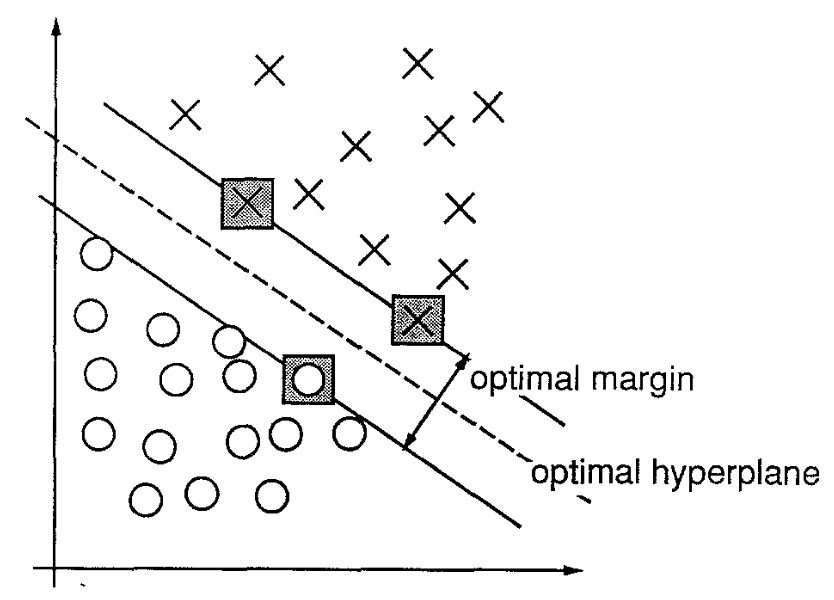
\includegraphics[width=.7\textwidth]{images/svm.png}
		\caption[An example of a \ac{SVM} in a two-category case]{An example of a \ac{SVM} in a two-category case, from \cite[p. 275]{Cortes1995}}
		\label{fig:background-optionmining-machinelearningalgorithms-svm}
	\end{figure}
	
\end{description}

\subsection{Metrics}
\label{ss:background-optionmining-metrics}

The performance of algorithms in \cref{ss:background-optionmining-machinelearningalgorithms} can be measured by some metrics.
In the following the most important metrics will be presented.

\begin{description}
	\item [Confusion Matrix]
		The confusion matrix shows the relation between correctly and wrongly predicted items.
		To build a confusion matrix each label is predicted by the algorithm and counted as follows:
		If the correct label is \emph{positive} and the algorithm predicted \emph{positive}, than it is a \ac{TP}.
		On the other hand if the algorithm predicted \emph{negative} it is a \ac{FN}.
		The same structure applies if the correct label is \emph{negative}: \ac{TN} if the algorithm predicted \emph{negative} and \ac{FP} if the algorithm predicted \emph{positive}
		\cite{Tripathy2015}.

		A sample confusion matrix is depicted in \cref{tab:background-optionmining-confusionmatrix}.

		Based on this confusion matrix some other metrics can be calculated.
		
		\begin{table}
			\begin{center}
				\begin{tabular}{l | l l}
					 & \multicolumn{2}{c}{Correct labels} \\
					Predicted labels & Positive & Negative \\ \hline
					Positive & \ac{TP} & \ac{FP} \\
					Negative & \ac{FN} & \ac{TN} \\ \hline					
				\end{tabular}
		
				\caption{A sample confusion matrix}
				\label{tab:background-optionmining-confusionmatrix}
			\end{center}
		\end{table}

	\item [Precision]
		Precision measures the exactness of the algorithm.
		It is the ratio of correctly predicted positive labels to the total number of items predicted as positive
		\cite{Tripathy2015}.

		\begin{equation}
			precision = \frac{\ac{TP}}{\ac{TP}+\ac{FP}}
			\label{eq:background-optionmining-metrics-precision}
		\end{equation}

	\item [Recall]
		Recall measures the completeness of the algorithm.
		It is the ratio of number of correctly predicted positive labels to the actual number of positive items present in the corpus
		\cite{Tripathy2015}.

		\begin{equation}
			recall = \frac{\ac{TP}}{\ac{TP}+\ac{FN}}
			\label{eq:background-optionmining-metrics-recall}
		\end{equation}

	\item [F-Measure]
		F-Measure is the harmonic mean of precision and recall.
		It has the best value at 1 and the worst value at 0
		\cite{Tripathy2015}.
		The formula is show in \cref{eq:background-optionmining-metrics-f_measure}.

		\begin{equation}
			F-Measure = \frac{2 * precision * recall}{precision + recall}
			\label{eq:background-optionmining-metrics-f_measure}
		\end{equation}

	\item [Accuracy]
		Accuracy is one of the most used metric for opinion mining algorithms.
		It is calculated as the ratio of number of correctly predicted items to the total number of available items in the corpus
		\cite{Tripathy2015}.

		\begin{equation}
			accuracy = \frac{\ac{TP} + \ac{TN}}{\ac{TP}+ \ac{TN} + \ac{FP} + \ac{FN}}
			\label{eq:background-optionmining-metrics-accuracy}
		\end{equation}

\end{description}

\section{Social networks/microblogging services}
\label{s:background-socialnetworks}

In the last years many social networks started and many of them disappeared again.
There are several types of social networks available today: some of them are built on videos others on pictures and some of them mostly on text.
Those which are built on text are more easy to analyze and searchable for researchers worldwide.
But there are some constants in this field: Twitter, to identify one of them.
Twitter has become a valuable source of opinions, data and information for various researches \cite{Barbosa2010}.

Messages on Twitter are called tweets and are limited in length (140 for tweets before \printdate{2017-11-07}; 280 characters since then, at least for english tweets \cite{Rosen2017}) and due to this fact users have to concentrate on a specific topic precisely.
Therefore, Twitter is the perfect source of the public opinion as users discussing anything on Twitter \cite{Pagolu2016a}.

As a result the fields in which researches have used data from Twitter ranging from public opinions for politicans and polls (see \cite{Oconnor2010a,Patodkar2016a}) to the stock market and the prediction of stock prices and other factors (see \cite{Bollen2011a,Mittal2012a,Nguyen2015a,Pagolu2016a,Zhang2011a}).

% On the other hand keywords like cloud, machine learning and artificial intelligence are everywhere. 
% Amazon, Facebook, Google, IBM and Microsoft and other big players of the industry are making massive progress in these fields.

\chapter{Experimental Setup}
    %!TEX root = ../main.tex

This chapter describes the setup of the case study.
The \cref{fig:casestudy-workflow} depicts the overall workflow of this thesis.
In the following sections each step is elucidated.
Strong emphasis is laid on numbers and decisions.

\begin{figure}[ht]
  \centering

  \smartdiagramset{back arrow disabled=true,
    text width=.6\textwidth,
    uniform color list=black!40 for 5 items}
  \smartdiagram[flow diagram:vertical]{
    {Determine companies, keywords and stock symbols to analyze},
    {Gather data},
    {Normalization of tweets},
    {Determine sentiment of tweets},
    {Comparing sentiment time series with share prices}
  }

  \caption{Workflow of this thesis}
  \label{fig:casestudy-workflow}
\end{figure}

\section{Determine Companies, Keywords and Stock Symbols to Analyze}
\label{s:casestudy-companieskeywords}

First, a list of automotive companies is needed.
These companies must be traded on a stock exchange to perform the comparison with tweet sentiments.
As a single company may own several car brands a list of all brands has been set up.
The result of the analysis is depicted in \cref{tab:casestudy-brands}.
Both brands which aren't customer facing passenger car brands and brands which do not longer exist have been omitted.
Furthermore, the brands have been grouped by their owning company.

  \begin{longtable}[c]{!l ^l}
    \hline
    \rowstyle{\bfseries}
    Car brand & Owning Company  \\ \hline
  \endfirsthead
  %
  \multicolumn{2}{c}%
  {{\bfseries Table \thetable\ continued from previous page}} \\
   &  \\
  \endhead
  %
  BMW  & BMW \cite[p.30]{BMWGroup2017} \\
  Mini  & BMW  \cite[p.30]{BMWGroup2017} \\
  Rolls-Royce   & BMW \cite[p.30]{BMWGroup2017} \\
  Mercedes-AMG & Daimler \cite[p.90]{DaimlerAG2018} \\
  Mercedes-Benz  & Daimler \cite[p.90]{DaimlerAG2018} \\
  Mercedes-Maybach & Daimler \cite[p.90]{DaimlerAG2018} \\
  Smart  & Daimler \cite[p.90]{DaimlerAG2018} \\
  Alfa Romeo & Fiat Chrysler Automobiles \cite[p.32]{FiatChryslerAutomobiles2018a} \\
  Chrysler & Fiat Chrysler Automobiles \cite[p.32]{FiatChryslerAutomobiles2018a} \\
  Dodge & Fiat Chrysler Automobiles \cite[p.32]{FiatChryslerAutomobiles2018a} \\
  Fiat & Fiat Chrysler Automobiles \cite[p.32]{FiatChryslerAutomobiles2018a} \\
  Fiat Professional & Fiat Chrysler Automobiles \cite[p.32]{FiatChryslerAutomobiles2018a} \\
  Jeep & Fiat Chrysler Automobiles \cite[p.32]{FiatChryslerAutomobiles2018a} \\
  Lancia & Fiat Chrysler Automobiles \cite[p.32]{FiatChryslerAutomobiles2018a} \\
  RAM & Fiat Chrysler Automobiles \cite[p.32]{FiatChryslerAutomobiles2018a} \\
  Ford & \ford\ \cite[p.18]{FordMotorCompany2018} \\
  Lincoln  & \ford\ \cite[p.18]{FordMotorCompany2018} \\
  Baojun & \gm\ \cite[p.1]{GeneralMotorsCompany2018} \\
  Buick & \gm\ \cite[p.1]{GeneralMotorsCompany2018} \\
  Cadillac & \gm\ \cite[p.1]{GeneralMotorsCompany2018} \\
  Chevrolet & \gm\ \cite[p.1]{GeneralMotorsCompany2018} \\
  GMC & \gm\ \cite[p.1]{GeneralMotorsCompany2018} \\
  Holden & \gm\ \cite[p.1]{GeneralMotorsCompany2018} \\
  Jiefang & \gm\ \cite[p.1]{GeneralMotorsCompany2018} \\
  Wuling & \gm\ \cite[p.1]{GeneralMotorsCompany2018} \\
  Honda & Honda \cite[p.3]{HondaMotorCo.2017} \\
  Hyundai & \hyundai\ \cite[p.127]{HyundaiMotorCompany2016} \\
  KIA & \hyundai\ \cite[p.127]{HyundaiMotorCompany2016} \\
  Datsun & Nissan Motor Corporation \cite[p.5]{NissanMotorCorporation2017} \\
  Infinity & Nissan Motor Corporation \cite[p.5]{NissanMotorCorporation2017} \\
  Nissan & Nissan Motor Corporation \cite[p.5]{NissanMotorCorporation2017} \\
  Citroën & Groupe PSA \cite[p.3]{GroupePSA2018} \\
  Opel & Groupe PSA \cite[p.3]{GroupePSA2018} \\
  Peugeot& Groupe PSA \cite[p.3]{GroupePSA2018} \\
  Vauxhall & Groupe PSA \cite[p.3]{GroupePSA2018} \\
  Alpine & Groupe Renault \cite[p.11]{GroupeRenault2018} \\
  Dacia & Groupe Renault \cite[p.11]{GroupeRenault2018} \\
  Lada & Groupe Renault \cite[p.11]{GroupeRenault2018} \\
  Renault & Groupe Renault \cite[p.10]{GroupeRenault2018} \\
  Renault Samsung Motors & Groupe Renault \cite[p.10]{GroupeRenault2018} \\
  Daihatsu & \toyota\ \cite[p.2]{ToyotaMotorCorporation2018} \\
  Lexus & \toyota\ \cite[p.2]{ToyotaMotorCorporation2018} \\
  Toyota & \toyota\ \cite[p.2]{ToyotaMotorCorporation2018} \\
  Audi & \vw\ \cite[p.104]{VolkswagenAktiengesellschaft2017} \\
  Bentley & \vw\ \cite[p.104]{VolkswagenAktiengesellschaft2017} \\
  Bugatti & \vw\ \cite[p.104]{VolkswagenAktiengesellschaft2017} \\
  Lamborghini & \vw\ \cite[p.104]{VolkswagenAktiengesellschaft2017} \\
  Porsche & \vw\ \cite[p.104]{VolkswagenAktiengesellschaft2017} \\
  Seat & \vw\ \cite[p.104]{VolkswagenAktiengesellschaft2017} \\
  Škoda & \vw\ \cite[p.104]{VolkswagenAktiengesellschaft2017} \\
  Volkswagen & \vw\ \cite[p.104]{VolkswagenAktiengesellschaft2017} \\ \hline
  
  \caption{Automotive brands and their corresponding owning company}
  \label{tab:casestudy-brands}
  \end{longtable}

According to the survey of \emph{World Motor Vehicle Production 2016} the biggest five car manufacturing companies are: Toyota, Volkswagen, Hyundai, General Motors and Ford \cite{OICA2016}.
Therefore the study will focus on these five companies.
The count of manufactured cars and the companies stock symbol are summarized in \cref{tab:casestudy-companies-counts-and-symbols}.
The containing symbols in the table are derived by literature research and using the Yahoo Finance portal (\url{https://finance.yahoo.com}).

\begin{table}
  \begin{tabular}[c]{!l ^r ^l ^l}
    \hline
    \rowstyle{\bfseries}
	  Company & \#cars \cite{OICA2016} & Stock Exchange & Symbol  \\ \hline
	  \ford\ & 6,429,485 & New York \cite{FordMotorCompany2018} & F  \\
	  \gm\ & 7,793,066 & New York \cite[p.17]{GeneralMotorsCompany2018} & GM \\
	  \hyundai\ & 7,889,538 & Korea \cite[p.92]{HyundaiMotorCompany2016} & 005380.KS \\
	  \toyota\ & 10,213,486 & Tokyo \cite{ToyotaMotorCorporation2018} & 7203.T \\
	  \vw\ & 10,126,281 & Frankfurt \cite[p.110]{VolkswagenAktiengesellschaft2017} & VOW.F \\  \hline
	\end{tabular}
	\caption{Automotive companies and their corresponding produced cars and stock symbol}
	\label{tab:casestudy-companies-counts-and-symbols}
\end{table}

\section{Gather Data}
\label{s:casestudy-gatherdata}

Gathering data is split into two different tasks:
gathering tweets which is described in detail in \cref{ss:casestudy-gatherdata-tweets}, 
and gather stock prices which is described in \cref{ss:casestudy-gatherdata-stockprices}.

\subsection{Gather Tweets}
\label{ss:casestudy-gatherdata-tweets}

A large set of tweets is needed to perform the analysis within a time frame of at least one month.
There were several approaches to get these tweets: download tweets directly or capture tweets within the given time frame.
As we are tracking five companies using 23 keywords (brands) there will be a quite big amount of data.

Several approaches have been tried to get as many tweets as possible to the given keywords, including:

\begin{description}
  \item [Official Twitter search \ac{API}] 
    was the first attempt.
    But there were very serious limitations to the official \ac{API} that made that quite easy way impossible.
    First, the standard search \ac{API} supports just a maximum count of 100 tweets;
    second, it supports a history of only seven days;
    and lastly, there were to tight rate limits defined in order gather all possible tweets of the seven days period \cite{TwitterInc.2018}.

  \item [Twitter search on website]
    has been tried to overcome the shortcomings of the official Twitter \ac{API} but the tweets cannot be downloaded in a easy way as the results only appear within the web browser.
    A Java tool (\url{https://github.com/Jefferson-Henrique/GetOldTweets-java}) has been found which tries to exploit the search page and extract tweets from the website.
    But this tool did not work as expected.
    Most likely Twitter made some changes to the search result page and the tool has not been adopted since \printdate{2016-04-15} \cite{Jefferson2016}.

  \item [DMI TCAT]
    is a toolset for capturing and analyzing tweets.
    It has been developed by \citeauthor{Borra2014} to support researchers around the globe and make tweet collection and analysis easier
    \cite{Borra2014}.
    TCAT support various ways of data capturing:
    \begin{itemize}
      \item One percent random sample of all tweets passing through Twitter,
      \item Streaming endpoint of the \ac{API} to track up to 400 keywords,
      \item Following up to 5000 specified users, such as members of a parliament or other expert lists \cite{Borra2014}.
    \end{itemize}

\end{description}

After exploring all of these methods DMI TCAT has been selected to capture the necessary Twitter data by using the streaming endpoint of the \ac{API} to track 23 keywords.
The tool must be installed on a computer in order to perform its work.
As the tool need some serious amount of capacities and need to collect tweets 24/7 it has been installed on a virtual machine in the Microsoft Azure cloud.

The 23 keywords have been grouped by the owning company into so called query bins.
A query bin may contain multiple keywords to track and combine all identified tweets into one single data set \cite{Borra2014}.

All tweets have been captured between \printdate{2018-02-28} to \printdate{2018-09-06}.
But there were several issues using the cloud approach:

\begin{itemize}

  \item By default the virtual machine in the cloud shut down every day on 7 PM.
    First a problem with the tool was expected but after several days and starting the virtual machine manually the origin of the issue was discovered and solved.

  \item The storage space of the virtual machine initialized with 30 \ac{GB}, which was too small for the collected tweet amount.
    The storage was full after approximately 14 days of data collection.
    As the problem was not detected right away it took several days for identifying and fixing the issue.

  \item The rate limits of the \ac{API} have been hit now and then in case too many tweets were published.
    DMI TCAT continued to collect tweets automatically after the corresponding time window.

  \item New releases DMI TCAT have been published from time to time which also required a database upgrade.
    As the performance was dropping the upgrade was performed in the hope of fixing the performance issue.
    Furthermore, the first update was needed to enable DMI TCAT to process tweets longer than 140 characters.
    The database upgrade needed to suspend the tweet collection by a serious amount of time.
    To collect as many tweets as possible the upgrade was performed in steps for each query bin separately.
    The larger the query bin the longer the process took as every single tweet was needed to be altered.

\end{itemize}

The number of collected tweets can be seen in \cref{tab:casestudy-companies-numberoftweets}.

\begin{table}[hbt]
  \centering
  \begin{tabular}{!l ^r ^r}
    \hline
    \rowstyle{\bfseries}
        Company   & \# captured tweets  & \# english tweets  \\ \hline
        \ford\    & \num{4518198}       & \num{3745447} \\  % has been 3745490
        \gm\      & \num{575547}        & \num{413817} \\
        \hyundai\ & \num{1895306}       & \num{697221} \\  % has been 697277
        \toyota\  & \num{915868}        & \num{488913} \\
        \vw\      & \num{8244083}       & \num{6219350} \\ \hline  % has been 6219786
        Total     & \num{16149002}      & \num{11565283} \\ \hline
  \end{tabular}

  \caption{Numbers of collected tweets}
  \label{tab:casestudy-companies-numberoftweets}
\end{table}

\subsection{Gather Stock Prices}
\label{ss:casestudy-gatherdata-stockprices}

The stock data can be downloaded at any point of time for the given research period on a daily frequency basis using the Yahoo Finance website.
The stock prices in a time frame of a year have been downloaded which contains the period of tweet collection.

The data contains the following information for each day:
Date, Open, High, Low, Close, Adj. Close and Volume.

% \begin{description}
%   \item [Date] on which the data applies
%   \item [Open]
% \end{description}

\section{Normalization of Tweets}
\label{s:casestudy-normalization}

Prior analysis the tweets have been preprocessed which is also called normalization.
The importance of normalization has been described in \cref{ss:background-optionmining-textfeatureextraction}.

In the following the steps of normalization are described in detail:

\begin{description}

  \item [Lower case:]
    The tweet text is converted to lower case as the meaning stays the same but the dictionary size is reduced.

  \item [Tokenization:]
    For tokenization the \emph{TweetTokenizer} of the NLTK package is used.
    This tokenizer has been created for this purpose.

  \item [Stopwords:]
    The predefined english stopwords of the NLTK package have been removed from all tweets.
  
  \item [Lemmatization:]
    There are several lemmatizer available and the \emph{WordNetLemmatizer} of the NLTK package is used to perform this step.

  \item [Stemming:]
    The same situation applies to stemmers.
    The \emph{SnowballStemmer} of the NLTK package is used as many found examples used this specific stemmer.

  \item [Custom \ac{RegEx}:]
    Last but not least, custom \ac{RegEx} have been used to remove or replace other unwanted elements of tweets, such as \cite{Pagolu2016a}:

    \begin{enumerate}
      \item User references (``@someuser'') are replaced with the generic word ``user''.
      \item Specific URI are replaced with the word ``uri''.
      \item Three or more consecutive characters are replaced by two consecutive characters.
        For example: the word ``coooooooool'' becomes ``cool''.
      %\item Questionmarks are replaced by the word ``question'' and exclamationmarks are replace by the word ``exclamation''.
      \item Hashtags have been removed as the hash symbol does not provide any additional information. 
        For example: the hashtag ``\#cool'' is replaced by ``cool''.
    \end{enumerate}

\end{description}

As these described normalization steps are language sensitive only english tweets are used for this and following steps.

\section{Determine Sentiment of Tweets}
\label{s:casestudy-sentiment}
% maybe useful?
% https://github.com/ayushoriginal/Sentiment-Analysis-Twitter

After normalization the tweets were ready for sentiment detection.
The sentiments were detected using four different classifiers using the same workflow depicted in \cref{fig:casestudy-sentimentworkflow}, the used symbols are described in \cref{tab:casestudy-sentimentvariables} and the same pipeline configuration depicted in \cref{fig:casestudy-sentimentpipeline}.

\begin{table}[hbt]
  \centering
  \begin{tabular}{!l ^l}
    \hline
    \rowstyle{\bfseries}
    Symbol & Description \\ \hline
    $T_S$ & Sample tweets \\
    $T_C$ & Collected tweets \\
    $P$   & Pipeline \\
    $P_T$ & Trained pipeline \\
    $S$   & Sentiment \\ \hline
  \end{tabular}

  \caption{Variable definitions for sentiment detection}
  \label{tab:casestudy-sentimentvariables}
\end{table}

\begin{figure}[hbt]
  \centering
  
  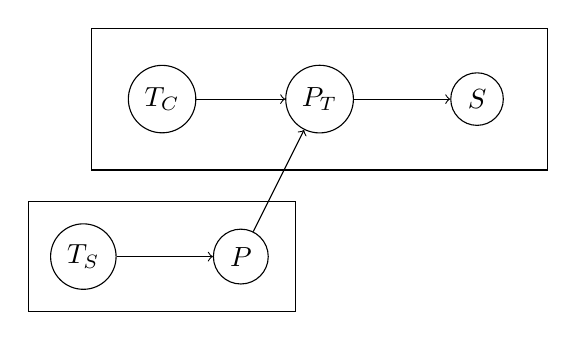
\begin{tikzpicture}
    \node (ts) at (0,0) [circle, draw] {$T_S$};
    \node (p) at (2,0) [circle, draw] {$P$};
    \node (tc) at (1,2) [circle, draw] {$T_C$};
    \node (pt) at (3,2) [circle, draw] {$P_T$};
    \node (s) at (5,2) [circle, draw] {$S$};

    \draw[->] (ts) -- (p);
    \draw[->] (tc) -- (pt);
    \draw[->] (p) -- (pt);
    \draw[->] (pt) -- (s);

    \draw (-.7,-.7) rectangle (2.7,.7);
    \draw (0.1,1.1) rectangle (5.9,2.9);
  \end{tikzpicture}

  \caption{Workflow for sentiment detection}
  \label{fig:casestudy-sentimentworkflow}
\end{figure}

\begin{figure}[hbt]
  \centering
  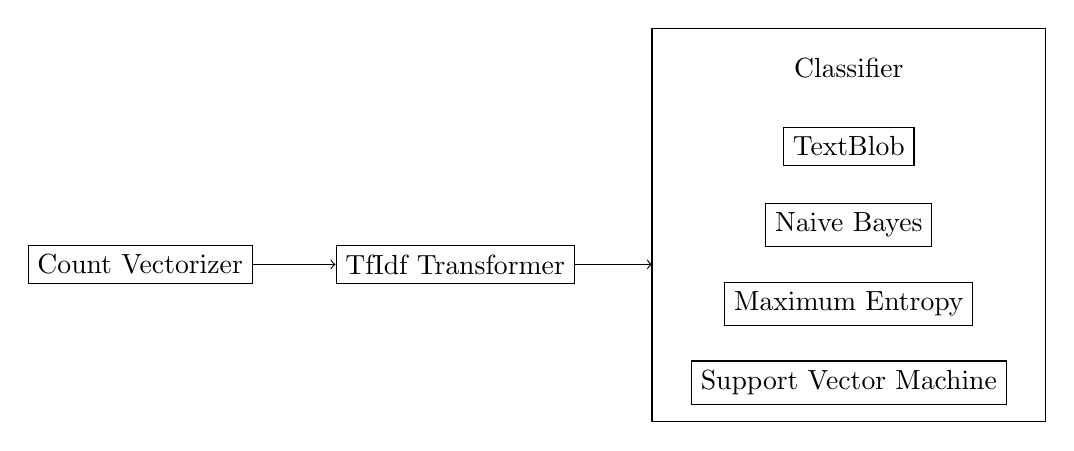
\begin{tikzpicture}
    \node (cv)     at (0,0) [rectangle, draw] {Count Vectorizer};
    \node (tfidf)  at (4,0) [rectangle, draw] {TfIdf Transformer};

    \node (cf_tb)  at (9,1.5) [rectangle, draw] {TextBlob};
    \node (cf_nb)  at (9,0.5) [rectangle, draw] {Naive Bayes};
    \node (cf_me)  at (9,-0.5) [rectangle, draw] {Maximum Entropy};
    \node (cf_svm) at (9,-1.5) [rectangle, draw] {Support Vector Machine};

    \node (cf)     at (9,2.5) {Classifier};
    
    \draw (6.5,-2) rectangle (11.5,3);

    \draw[->] (cv) -- (tfidf);
    \draw[->] (tfidf) -- (6.5,0);
  \end{tikzpicture}

  \caption{Pipeline for sentiment detection}
  \label{fig:casestudy-sentimentpipeline}
\end{figure}

%buitinck2013api

Pipelines are a useful construct provided by the \emph{scikit-learn} project.
The basic philosophy in this project is to divide the public \ac{API} into four parts:

\begin{description}
  \item [Data representation.]
    In most machine learning tasks the data is modeled as a set of variables.
    In supervised learning tasks the goal is to find a mapping from various input variables to some output variables.
    A common way to represent such a dataset is a pair of matrices: one for the input values and one for the output values.
    Within one matrix one column corresponds to one variable and one row corresponds to a specific sample of the problem.
    To construct such matrices from textual data \emph{scikit-learn} provides \emph{vectorizer} objects
    \cite{buitinck2013api}.

  \item [Estimators.]
    Machine learning tasks are designed as \emph{estimator} objects which expose a \emph{fit} method.
    It provides the separation of model creation and learning.
    A model is initialized with specific parameters regarding the specific task which are also called \emph{hyper-parameters}.
    The actual learning is provided by the \emph{fit} method which takes two matrices as input parameters at least for supervised learning algorithms.
    After fitting the parameters to the training data the model is trained and can be used to perform predictions or transformations
    \cite{buitinck2013api}.

  \item [Predictors.]
    \emph{Predictors} are used to produce target variables by a given set of input variables.
    The \emph{predict} method is also supplied by the same model object which has been trained before by using the \emph{fit} method.
    Beside the \emph{predict} method predictors have to provide a \emph{score} method which quantifies the quality of the predictions.
    For supervised learning models the \emph{score} method takes two matrices as input parameters: input data and expected output data.
    Using the import data the model then predicts the output values and calculates the difference to the expected output values.
    The higher the calculated score is the better is the quality of the prediction
    \cite{buitinck2013api}.

  \item [Transformers.]
    Usually data is modified or filtered before it is used for model training or prediction.
    Therefore \emph{scikit-learn} provides objects with the \emph{transformer} interface which exposes a method called \emph{transform}.
    The method takes an input parameter for input values and generates a transformed matrix of input values.
    \emph{Transformers} can be used to scale values to the standard normal distribution
    \cite{buitinck2013api}.

\end{description}

\emph{Scikit-learn} provides furthermore a mechanism to combine several estimators to a new estimator which than can be used such as a basic estimator.
To provide a simple sequential workflow of feature extraction, transforming, fitting and prediction \emph{scikit-learn} provides pipeline objects.
The pipeline is a useful construct to perform the same steps over and over in a standardized way for training and estimation
\cite{buitinck2013api}.

% Cross validation with GridSearchCV
Furthermore \emph{scikit-learn} provides some helpers to find the best hyper-parameters for the given problem.
The user can define which values various hyper-parameters can attain and the helper then perform test runs for various combinations, calculate their score and keep acting as the best performing model.
Therefore, this type of search is called \emph{model selection}.
\emph{Scikit-learn} provides two different model selection helpers: \emph{GridSearchCV} and \emph{RandomizedSearchCV}.
Whereas \emph{GridSearchCV} generates a \emph{grid} of the complete combinatorial combinations and perform the scoring with every single combination, \emph{RandomizedSearchCV} takes a fixed number of parameter combinations
\cite{buitinck2013api}.

The model selection helper of \emph{scikit-learn} can also perform a cross-validation.
By default \emph{GridSearchCV} uses \emph{k-fold} cross-validation by optimizing the \emph{score} function of the estimator.
The value which should be optimized can be changed to a variety of predefined key figures including the $F-Measure$
\cite{buitinck2013api}.

In this thesis the \emph{GridSearchCV} model selection helper is used. 
In the following sections each part of the pipeline and tried hyper-parameters used are described.

\begin{description}
  \item[Count Vectorizer] 
    The count vectorizer is used to generate both a vocabulary and a numerical representation of the normalized tweets.
        
    \begin{table}[!hbt]
      \centering
      \begin{tabular}{!l ^l}
        \hline
        \rowstyle{\bfseries}
        Variable & Tried values \\ \hline
        NGrams & 1-gram to 4-grams \\
        Stopwords & none \\
        Binary & true, false \\ \hline
      \end{tabular}
    
      \caption{Hyper-parameters of the CountVectorizer}
      \label{tab:casestudy-hyperparams-countvectorizer}
    \end{table}
  

  \item[\ac{TF-IDF} Transformer]
    The \ac{TF-IDF} is used to transform the vocabulary from the count vectorizer to make common words less important for the analysis.
    The implementation used also supports to deactivate the transformation at all.
    If the untransformed vocabulary would lead to better results the GridSearchCV would figure that out and use the best set of parameters.
    All hyper-parameters for the transformer can be found in \cref{tab:casestudy-hyperparams-tfidftransfomer}.
  
    \begin{table}[!hbt]
      \centering
      \begin{tabular}{!l ^l}
        \hline
        \rowstyle{\bfseries}
        Variable & Tried values \\ \hline
        Use IDF & true, false \\
        Smooth IDF & true \\
        Normalization & 'l1', 'l2', none \\ \hline
      \end{tabular}
    
      \caption{Hyper-parameters of the \ac{TF-IDF} Transformer}
      \label{tab:casestudy-hyperparams-tfidftransfomer}
    \end{table}
  
    
  \item[Classifier]
    The pipeline has been tried using four different classifiers.
    Each of them has different hyper-parameter.
    Therefore, they will be discussed in the corresponding sections.

    \begin{description}
      \item[TextBlob Classifier]
      
        The TextBlob classifier is a pre-trained classifier which has no hyper-parameters at all.
        It works out of the box.
        The only effort made was to make the TextBlob classifier available to the scikit-learn package by implementing the estimator interface (the method \emph{predict}).
        
      \item[Naive Bayes Classifier]
        The Naive Bayes classifier was the first classifier which supported hyper-parameters.
        As the philosophy of \emph{scikit-learn} is to provide good default values only some hyper-parameters have been modified
        \cite{buitinck2013api}.
        The implementation used is class \emph{sklearn.naive\_bayes.MultinomialNB}.
        All tried hyper-parameter values are depicted in \cref{tab:casestudy-hyperparams-nbclassifier}.
      
        \begin{table}[!hbt]
          \centering
          \begin{tabular}{!l ^l}
            \hline
            \rowstyle{\bfseries}
            Variable & Tried values \\ \hline
            Alpha & $10^{-2}$, $10^{-3}$ \\ \hline
          \end{tabular}
        
          \caption{Hyper-parameters of the Naive Bayes Classifier}
          \label{tab:casestudy-hyperparams-nbclassifier}
        \end{table}
        
      \item[Maximum Entropy Classifier]
        The implementation used for the Maximum Entropy classifier is class \emph{sklearn.linear\_model.LogisticRegression} which have some built in solvers.
        The tried solvers and other hyper-parameters can be found in \cref{tab:casestudy-hyperparams-meclassifier}.
      
        \begin{table}[!hbt]
          \centering
          \begin{tabular}{!l ^l}
            \hline
            \rowstyle{\bfseries}
            Variable & Tried values \\ \hline
            Solver & 'liblinear', 'lbfgs', 'sag', 'saga' \\
            Multiclass & 'auto' \\ \hline
          \end{tabular}
        
          \caption{Hyper-parameters of the Maximum Entropy Classifier}
          \label{tab:casestudy-hyperparams-meclassifier}
        \end{table}
        
      \item[Support Vector Machine Classifier]
        The Support Vector Machine classifier used is class \emph{sklearn.linear\_model.SGDClassifier} with loss function 'hinge' as this is the only support loss function which results in a linear \svm.
        Other hyper-parameters can be found in \cref{tab:casestudy-hyperparams-svmclassifier}.
      
        \begin{table}[!hbt]
          \centering
          \begin{tabular}{!l ^l}
            \hline
            \rowstyle{\bfseries}
            Variable & Tried values \\ \hline
            Tolerance & $10^{-2}$, $10^{-3}$ \\
            Loss & 'hinge' \\ \hline
          \end{tabular}
        
          \caption{Hyper-parameters of the Support Vector Machine Classifier}
          \label{tab:casestudy-hyperparams-svmclassifier}
        \end{table}
        
    \end{description}

    A pipeline is built for each classifier.
    The GridSearchCV model selector is used to train the specific pipeline using the hyper-parameters defined to find the best possible parameters for each component.

    The sentiment analysis is then performed with the selected model and stored in files for further analysis.

  \item[Comparing Sentiment Time Series with Share Prices]
    
    Both datasets, stock prices and sentiment analysis results respectively, are stored in files prior the comparison.
    The stock prices are already in a time series format on a daily basis except for weekends or holidays but the problem of missing entries are tackled later.
    First, the sentiment analysis result dataset must be condensed to form a time series for comparison.
    Therefore the results per tweet are grouped per day and summed up.
    As negative sentiments have the value \texttt{'-1'} and positive sentiments have the value \texttt{'1'} we receive a number which is positive in case more positive than negative tweets have been published on that given day and vice versa. 

    Missing stock prices have been calculated iteratively and the gaps have been filled by using the following procedure:
    Given $x$ is a stock price value and $y$ is the next present value with one or more values in between are missing.
    The missing values are calculated using the formula $\frac{x+y}{2}$.
    The formula is applied to the first missing value then the calculated value is treated as new $x$ and so on.
    These steps are repeated as long values were missing
    \cite{Pagolu2016a}.

    As there were several phases were no tweets have been tracked only consecutive time series of at least five days have been taken into account for further analysis.

\end{description}

\chapter{Conclusion}
    This final section provides a short summary of literature research, analysis and comparison in \cref{s:conclusions-summary}.
\Cref{s:conclusions-discussion} discusses the results critically and shows up limitations and shortcomings. 
Finally, \cref{s:conclusions-future} provides possible future research topics.

\section{Summary of Results}
\label{s:conclusions-summary}

\rework{
The central research question stated in \cref{s:introduction-researchgoals} was: \emph{To what extent can stock market movements be explained by the public opinion extracted from Twitter?}

We evaluated that the best results are achieved using all tweets (no tweets omitted), \svm{} or \nb{} classifier and a lag between five and nine days.

In the following we recall all defined research goals in \cref{s:introduction-researchgoals} on page \pageref{s:introduction-researchgoals} and give an answer to these.}
In the following each research goal is stated and a short summary of the results is given in each subsection.

% research goals

\subsection{G1 - Determine Companies, Keywords and Stock Symbols to Analyze}
\label{ss:conclusion-summary-g1}

% \item \textbf{G1-Q1} - Which companies should be analyzed?
% \item \textbf{G1-Q2} - Which keywords should be used to find corresponding tweets?
% \item \textbf{G1-Q3} - Which company uses which stock symbol in order to retrieve share prices?

The research goal 1 has been answered in \cref{s:casestudy-companieskeywords} (see page \pageref{s:casestudy-companieskeywords}).
In the following a short summary is given.
First the question of which companies should be analyzed must be answered.
In literature there were many references to automotive companies and therefore the decision has been made to analyze these companies.
To find the corresponding companies the five biggest car manufacturing companies have been selected.
This selection has been made based on the survey \emph{World Motor Vehicle Production 2016} \citep{OICA2016}. 
The resulting companies are depicted in \cref{tab:casestudy-brands}.

Secondly, a list of keywords must be composed in order to search for tweets for the specific companies.
As these companies own several customer facing car manufacturing brands these will be used as keywords too.
Therefore, the \cref{tab:casestudy-brands} also contains all customer facing car manufacturing brands for the top five companies.

Thirdly, the companies must be traded on any stock exchange market and we have to research the stock symbols and the market in order to retrieve their stock prices.
The results of this research are depicted in \cref{tab:casestudy-companies-counts-and-symbols}.

\subsection{G2 - Gather Tweets and their Sentiments and Stock Prices}
\label{ss:conclusion-summary-g2}

% \item \textbf{G2-Q4} - Why Twitter and not anything else? (2.3)
% \item \textbf{G2-Q5} - In which way tweets can be collected?
% \item \textbf{G2-Q6} - In which way sentiments can be determined?
% \item \textbf{G2-Q7} - Which sentiments are present for various companies?

The research goal 2 consists of four research questions.
First the decision for using Twitter as social media platform of our choice has been made as the characters are limited for each post and therefore the probability of a single topic per tweet is higher than on other platforms.
Furthermore, several other papers in literature have been using Twitter as reliable source.
This has been discussed in \cref{s:background-socialnetworks}.

Secondly, there is the questions how tweets can be collected from twitter which has been answered in \cref{ss:casestudy-gatherdata-tweets}.
Three different possibilities of tweet collection could be identified:

\begin{description}
    \item[Official Twitter Search \ac{API}]
        follows the pull principle. 
        The user requests something and the \ac{API} sends a response.
        But there were some serious limitations which caused that this way cannot be used.

    \item[Twitter search on website]
        does not have these limitations as the search \ac{API}.
        But it is no easy task to download and save search results from the official Twitter page.
        Therefore, also this possibility has been omitted due the difficulties.    
    
    \item[\ac{DMITCAT}] 
        is a toolset for capturing and analyzing tweets.
        It follows a different approach than the search \ac{API}.
        It supports the official streaming \ac{API} which follows a push principle and enables its users to capture tweets using up to 400 keywords.
        Therefore, the decision has been made to use \ac{DMITCAT} to capture tweets.

\end{description}

Thirdly, research has been made in which way sentiments can be determined (see \cref{s:casestudy-normalization} and \cref{s:casestudy-sentiment} for more details).
Most sentiment detection algorithms are performing their work better if the text source has been normalized in some way.
Normalization includes lower casing of text, applying stopwords, lemmatization, stemming and minor enhancements.
All of these normalization techniques have been applied to the collection of tweets which was a quite time consuming task as there were over 16 million tweets captured (see \cref{tab:casestudy-companies-numberoftweets}).

Four sentiment detection algorithms have been selected for the case study: \tb{}, \nb{}, \me{} and \svm{}.
In order to standardize the training and classification of each algorithm the \emph{scikit-learn} framework has been used.
The framework includes all algorithms and a so called \emph{pipeline} to perform this standardization for training and classification purposes.
The full script to train and analyze tweet sentiments can be found in the appendix (see \cref{lst:appendix-tweeets_analyzer}).

Fourthly, an analysis has been performed which sentiments are present in which company.
This is done in \cref{s:analysis-sentiments} beginning on page \pageref{s:analysis-sentiments}.
An overview of the tweet sentiments are depicted in \cref{tab:analysis-sentiments-general}.
It is shown that almost \SI{75}{\percent} of all tweets were rated as positive across all classifiers but there are differences in percentages by classifiers and company.
The \tb{} classifier for example is very optimistic whereas the \nb{} classifier is relatively pessimistic.
The same holds true for certain companies: \SI{80}{\percent} of all \gm{} tweets were positive whereas only $\frac{2}{3}$ of \vw{} tweets were positive.

\subsection{G3 - Comparing Sentiment Time Series with Share Prices}
\label{ss:conclusion-summary-g3}

% \item \textbf{G3-Q8} - Can the time series of sentiments explain the share prices?

% company      SA_TB.x SA_TB.y SA_NB.x SA_NB.y SA_ME.x SA_ME.y SA_SVM.xSA_SVM.ySA_TB   SA_NB   SA_ME   SA_SVM  RT      NoRt    total   count
% <chr>        <int>   <int>   <int>   <int>   <int>   <int>   <int>   <int>   <int>   <int>   <int>   <int>   <int>   <int>   <int>   <int>
% 1Ford           0       0       1       1       0       0       0       0       0       2       0       0       1       1       2      80
% 2GM             5       1       6       9       1       3       5       7       6      15       4      12      17      20      37      80
% 3Hyundai        7       8       7       0       7       1       7       1      15       7       8       8      28      10      38      80
% 4Toyota         0       0       0       0       0       0       0       0       0       0       0       0       0       0       0      80
% 5VW             0       6       6       1       0       1       9       3       6       7       1      12      15      11      26      80
%                12      15      20      11       8       5      21      11      27      31      13      32      61      42     103     400

In \cref{s:analysis-granger} the time series are compared to each other using the Granger analysis.
It tries to find a relation between the time series using a lag (in days).
In total 400 tests are performed: five companies for lags from one to ten days and four different sentiment classifiers using two different datasets (one with all tweets and one with omitted retweets).
The results are depicted in \rework{\cref{tab:analysis-classifiercomparision-summary}}.
From this 400 performed test 103 were significant.
It is shown that omitting \acp{RT} had a negative effect on the results (61 significant tests using all tweets versus 42 significant tests with omitted \acp{RT}).
For the company \ford{} only one classifier yield to a significant result (\fnb{} with both datasets).
But for the company \toyota{} not a single setup resulted in a significant result.

\section{Discussion and Limitations}
\label{s:conclusions-discussion}

This thesis tried to focus on five automotive companies but there were several difficulties during execution which leads to several limitations.

The first limitation is Twitter as datasource.
As the official search \ac{API} proved to be insufficient as there are some understandably limits in place the \ac{DMITCAT} approach was a good decision.
But using \ac{DMITCAT} had also some serious drawbacks:

\begin{itemize}
    \item 
        The software must be installed by one self and the machine must be up and running to collect tweets.
        As we can't keep the personal computer running continuously for more than one month we decided to install \ac{DMITCAT} to a virtual machine in the cloud.
        This decision yielded to several other problems:

        \begin{itemize}
            \item 
                The capacity of the provided virtual machine was way to small as 30 \ac{GB} of data has been captured within 14 days.
            \item 
                The virtual machine shut down every day on 7 PM. 
                Therefore several tweets were not captured at all.
            \item 
                New \ac{DMITCAT} releases have been published which required a database upgrade.
                This was a quite time consuming task and required that collection for the specific query bin is stopped.

            \item
                The excerpt of the collected data which was needed to perform the analysis need over 4 \ac{GB} in compressed size.
        \end{itemize}

    \item
        \ac{DMITCAT} uses also the official Twitter \ac{API} and as a result some limits apply.
        These limits have been hit from time to time and forced the tweet collection to pause.
        But the software continued to collect tweets automatically after the corresponding time window.
\end{itemize}

Second, the resulting gaps from data collection in the tweet time series resulted in fragmented data which made it pretty hard to analyze.
Maybe the results would be more precise if this gaps could be removed.

Third, the training of the sentiment classifiers used the Twitter corpus of \ac{NLTK} which contains each 5000 positive and 5000 negative tweets.
To improve the accuracy of the classifiers the training data could be extracted from the collected tweets which would require manual rating of the training set.

From these limitations the area for improvement for future research can be deducted.
Particularly the gaps in the twitter time series could seems to be a serious problem which make some statistical analysis unreliable.

\section{Future Research}
\label{s:conclusions-future}

% Future work:
% Issues with DMI TCAT (no gaps!)
% sarcasm in tweets
% retweets?
% classification in positive, neutral and negative?

This thesis at hand provides a basis to build on for upcoming researches and further points of interest can be deducted from the results of the study and the pointed out limitations.

First, the issues with the installation and maintenance of \ac{DMITCAT} need to be solved.
As the issues were technical they should be easy to solve by providing a computer with more resources which can run 24/7 for several months.
Furthermore, the collected data need serious amount of disk space and the sentiment classification algorithms need computation power and a fast hard disk.
This would also overcome the limitation of download the collected tweets from a virtual machine in order to analyze them.

Secondly, the classifiers have been trained to rate tweets binary (positive or negative).
In literature some also experimented with a trinary rating (positive, neutral or negative) which may lead to new conclusions.

Thirdly, the performed text pre-processing was a mixture of several approaches in literature.
This can be more fine grained especially for identifying sarcasm, slang and abbreviations within tweets.
Therefore, more research is needed to fine tune the text pre-processing and classification algorithms.
    
        %%------------------------END MATTER----------------------------%%
        %%--------------------------------------------------------------%%

\backmatter
        
\printbibliography[title={References}]
%\addcontentsline{toc}{chapter}{References}

\appendix
\chapter{Appendix A: Sentiment Analysis Python Script}
\chapter{Appendix A: Used Software, Packages and their Version}
  \begin{table}
    \centering
    \begin{tabular}[hbt]{!l ^l ^l}
      \hline
      \rowstyle{\bfseries}
      Used software & Package & Version \\ \hline
      Python &  & 3.7.2 \\
        & NLTK    & 3.3 \\
        & Numpy   & 1.15.4 \\
        & Pandas  & 0.23.4 \\
        & Python-dateutil & 2.7.5 \\
        & SciKit-Learn & 0.20.0 \\
        & SciPy   & 1.1.0 \\
        & TextBlob & 0.15.1 \\
        & TwitterAPI & 2.5.4 \\ \hline
      R & & 3.5.2 \\
        & dplyr & 0.7.8 \\
        & imputeTS & 2.7 \\
        & ggplot2 & 3.1.0 \\
        & fUnitRoots & 3042.79 \\
        & urca & 1.3.0 \\
        & vars & 1.5.3 \\
        & aod & 1.3 \\
        & zoo & 1.8.4 \\
        & tseries & 0.10.46 \\
        & tictoc & 1.0 \\ \hline
    \end{tabular}
  
    \caption{Used software and their corresponding version}
    \label{tab:casestudy-usedsoftware}
  \end{table}

\chapter{Appendix B: Sentiment Analysis Python Script}
%\lstinputlisting[language=Python, firstline=37, lastline=45]{source_filename.py}
\lstinputlisting[language=Python,caption={Python script for sentiment analysis of tweets},label=lst:appendix-tweeets_analyzer]{./code-files/tweets_analyzer.py}


% \chapter{List of installed software at FH Wiener Neustadt}
% 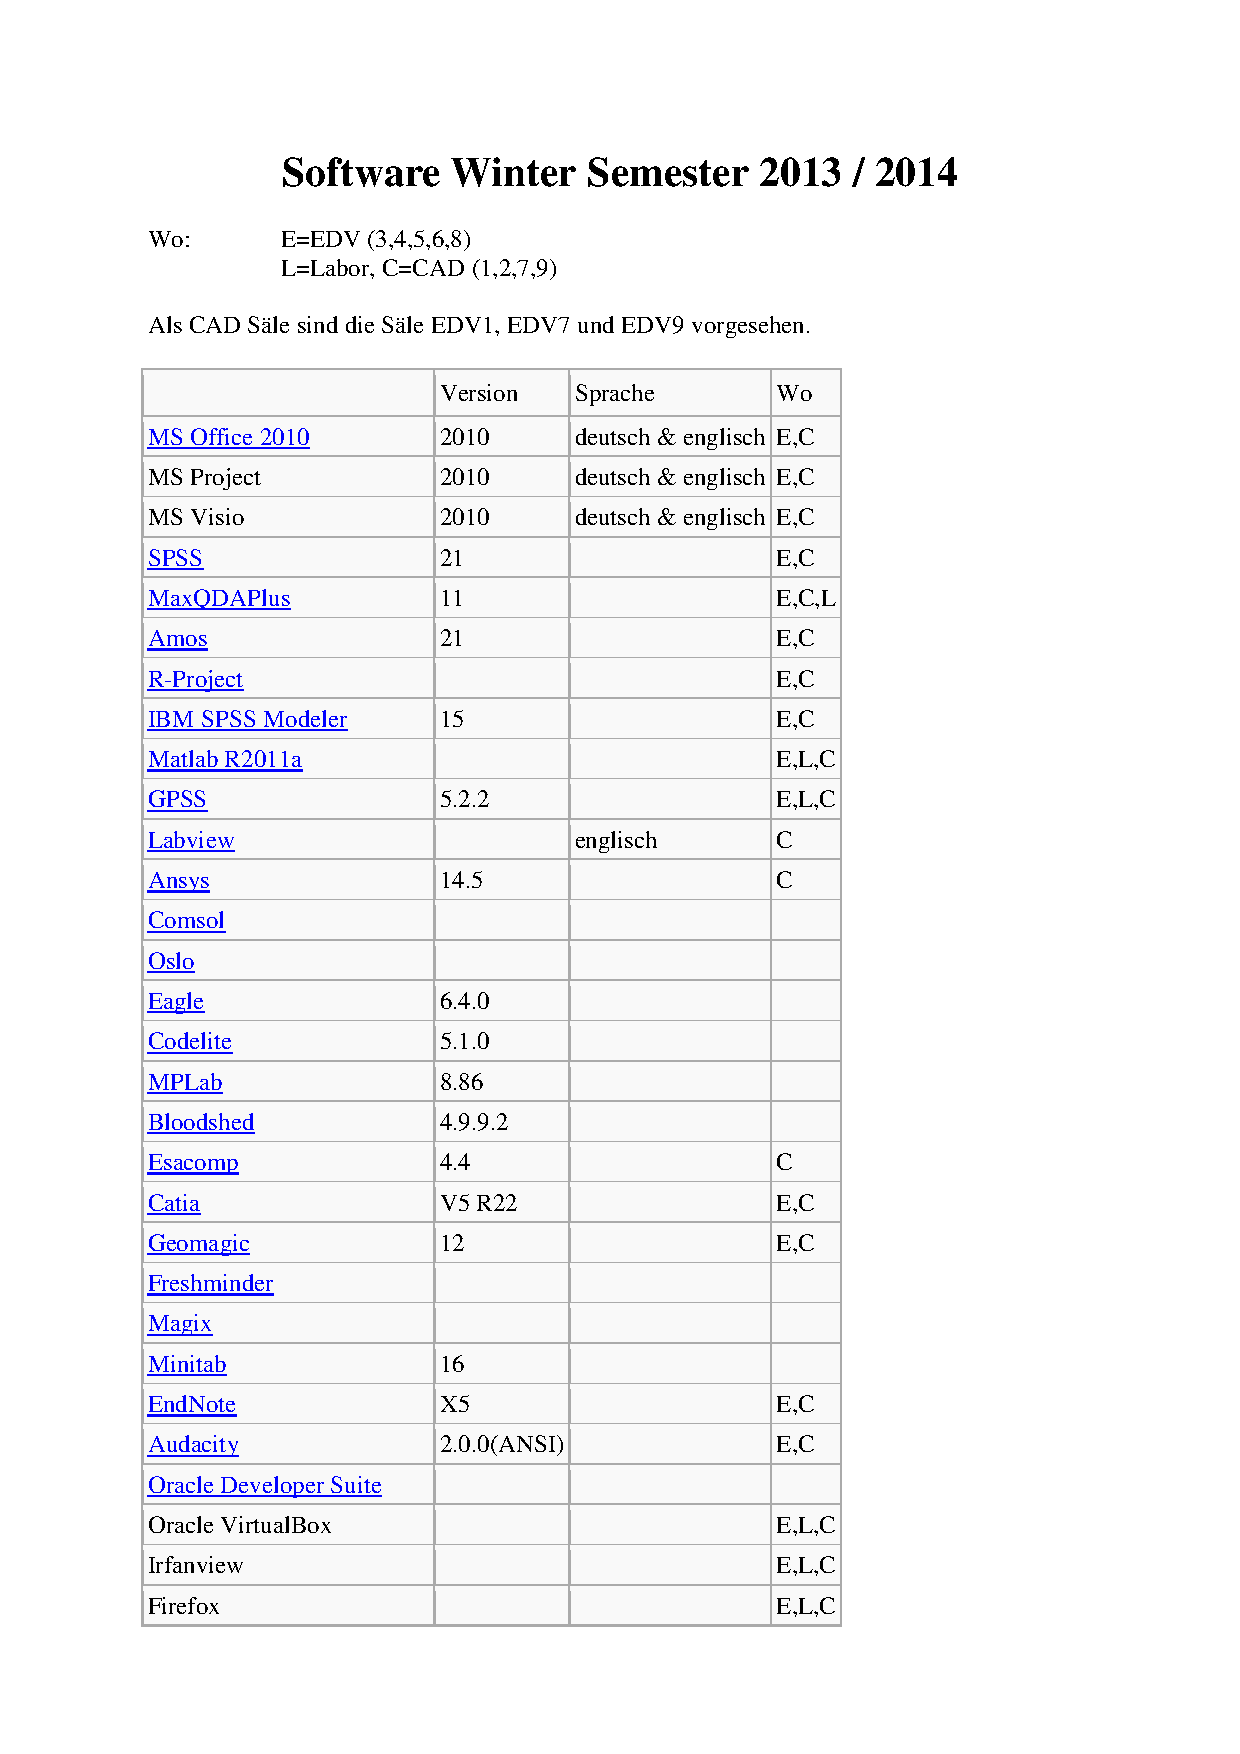
\includepdf[pages={1,2}]{externaldocs/itsoftware}

\end{document}